\documentclass{standalone} 
\PassOptionsToPackage{usenames,dvipsnames,svgnames}{xcolor}  
\usepackage{tikz}
\usetikzlibrary{arrows,positioning,automata,calc}

\begin{document}
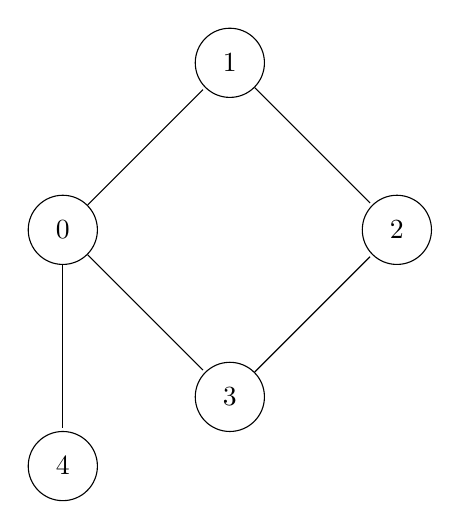
\begin{tikzpicture}[>=stealth',shorten >=1pt,node distance=3cm,on grid,initial/.style    ={}]
  \node[state]          (0)                          {0};
  \node[state]          (1)  [above right of = 0]    {1};
  \node[state]          (2)  [below right of = 1]   {2};
  \node[state]          (3)  [below right of = 0]   {3};
  \node[state]          (4)  [below       of = 0]   {4};

  \path (0)     edge [-]                    node   {} (4);
  \path (0)     edge [-]                    node   {} (1);
  \path (0)     edge [-]                    node   {} (3);
  \path (1)     edge [-]                    node   {} (2);
  \path (3)     edge [-]                    node   {} (2);

\end{tikzpicture}
\end{document}